\documentclass[11pt]{article}
\usepackage{amsmath,amssymb}
\usepackage{tikz}
\usetikzlibrary{arrows.meta,positioning}
\begin{document}
\title{T017 Dependency Map}
\author{Internal review packet}
\date{2026-06-18}
\maketitle
\begin{center}
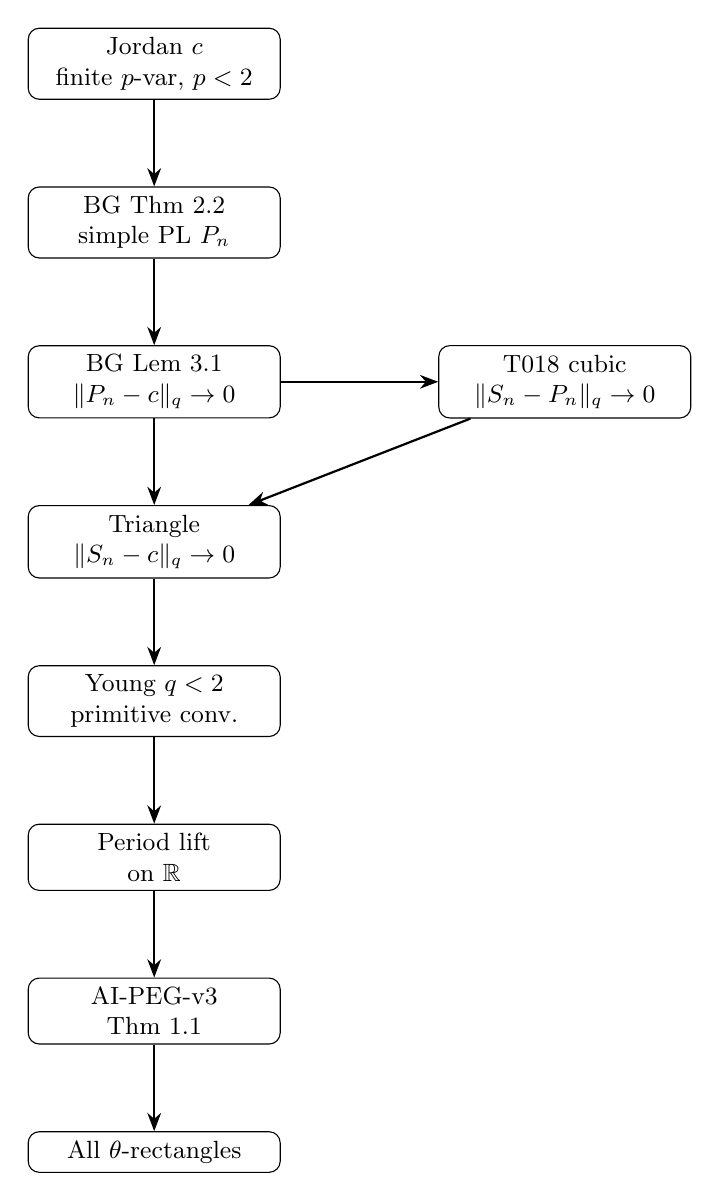
\begin{tikzpicture}[
  node distance=1.1cm and 2cm,
  box/.style={draw, rounded corners, align=center, minimum width=3.2cm, font=\small},
  arr/.style={-{Stealth}, thick}
]
\node[box] (c) {Jordan $c$\\ finite $p$-var, $p<2$};
\node[box, below=of c] (bg) {BG Thm 2.2\\ simple PL $P_n$};
\node[box, below=of bg] (bgL) {BG Lem 3.1\\ $\|P_n-c\|_{q}\to 0$};
\node[box, right=of bgL] (t18) {T018 cubic\\ $\|S_n-P_n\|_{q}\to 0$};
\node[box, below=of bgL] (tri) {Triangle\\ $\|S_n-c\|_{q}\to 0$};
\node[box, below=of tri] (young) {Young $q<2$\\ primitive conv.};
\node[box, below=of young] (lift) {Period lift\\ on $\mathbb R$};
\node[box, below=of lift] (ai) {AI-PEG-v3\\ Thm 1.1};
\node[box, below=of ai] (out) {All $\theta$-rectangles};
\draw[arr] (c) -- (bg);
\draw[arr] (bg) -- (bgL);
\draw[arr] (bgL) -- (t18);
\draw[arr] (bgL) -- (tri);
\draw[arr] (t18) -- (tri);
\draw[arr] (tri) -- (young);
\draw[arr] (young) -- (lift);
\draw[arr] (lift) -- (ai);
\draw[arr] (ai) -- (out);
\end{tikzpicture}
\end{center}
\end{document}
